\section{Introduction}\label{6sec:intro}


A Smart City is only useful if there are people who benefit from it.
There are a huge number of ways people interact with their city.
This part of this Smart City Concept tried to model 
one of the most frequent interactions, driving a car.
Thankfully, even as the number of vehicles in Germany grows\cite{carStat},
the number of accident fatalities continues to decrease.\cite{destatisCar}
As seen in Figure \ref{6fig:trend}, 
there were multiple measures done throughout recent history, 
to significantly the number of fatalities. 

\begin{figure}[H]
  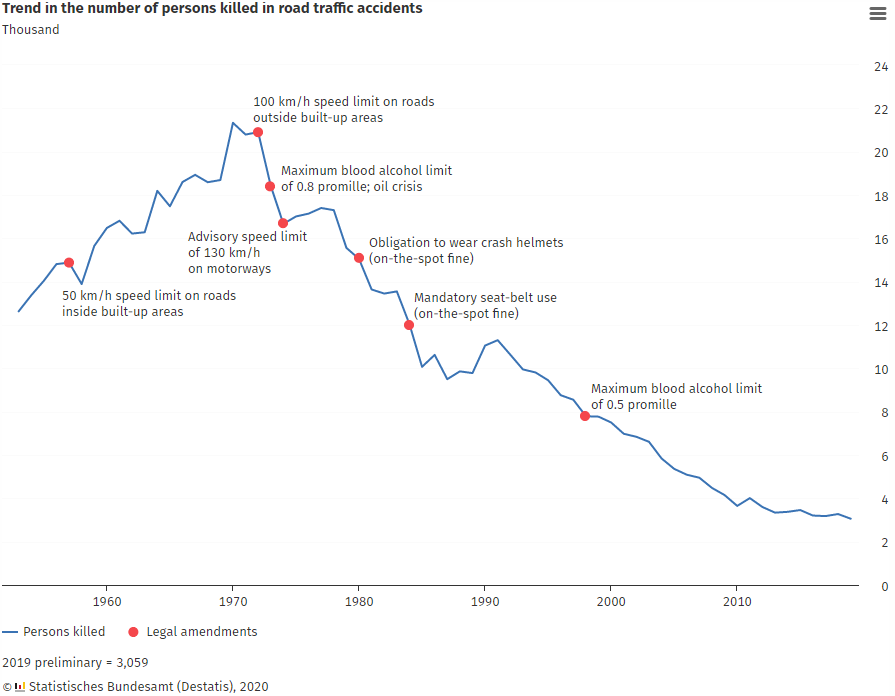
\includegraphics[width=0.9\linewidth]{chapters/chapter6_bruno/Figures/trendV2.png}
  \caption{Car Accident Trend \cite{destatisCar}}
  \label{6fig:trend}
\end{figure}

\noindent
But the decline has stagnated which still leaves around 3000 deaths a year in Germany.
Aside from the measures seen in Figure \ref{6fig:trend}, 
which try to keep accidents from happening, 
there is also another way to potentially save lives.
If the response from medical and police forces to an accident can be improved,
fewer accidents might lead to deaths. 
\\
\newline
This is what this part of the project was about. 
The goal was to connect all cars to the central server of the city.
These cars should always listen to their various sensors
and send a notification to the server
in case of an emergency.
Those emergencies are a physical crash or 
a sudden abnormality in the vitals of the driver.
\\
\newline
To simulate all this, the open source software CARLA was used.\footnote
{https://carla.org} 
CARLA is mostly used for traffic simulation and to develop autonomous driving prototypes,
but for this project, 
it served as a way to visualise the car crashes and the entire Smart City.
\\
\newline
The source code and an installation guide for this part of the project
can be found on GitHub.\footnote
{https://github.com/BrunoBerger/Connected-Vehicles}
The concept and the requirements can also be found
in the Wiki of the repository.